% Autor: Elias Welt
\section{Entstehung der Idee}

Die konzeptionelle Grundlage von EduShelf resultiert aus einer systematischen Analyse des schulischen Arbeitsalltags. Im Zuge der Beobachtung eigener Lernprozesse sowie der Erfahrungen aus dem Schulbetrieb kristallisierten sich wiederkehrende Ineffizienzen heraus, die als Ausgangspunkt für die Produktentwicklung dienten. Nachfolgend wird der ideelle Entstehungsprozess anhand von vier aufeinander aufbauenden Erkenntnisstufen erläutert.

\begin{figure}[h]
    \centering
    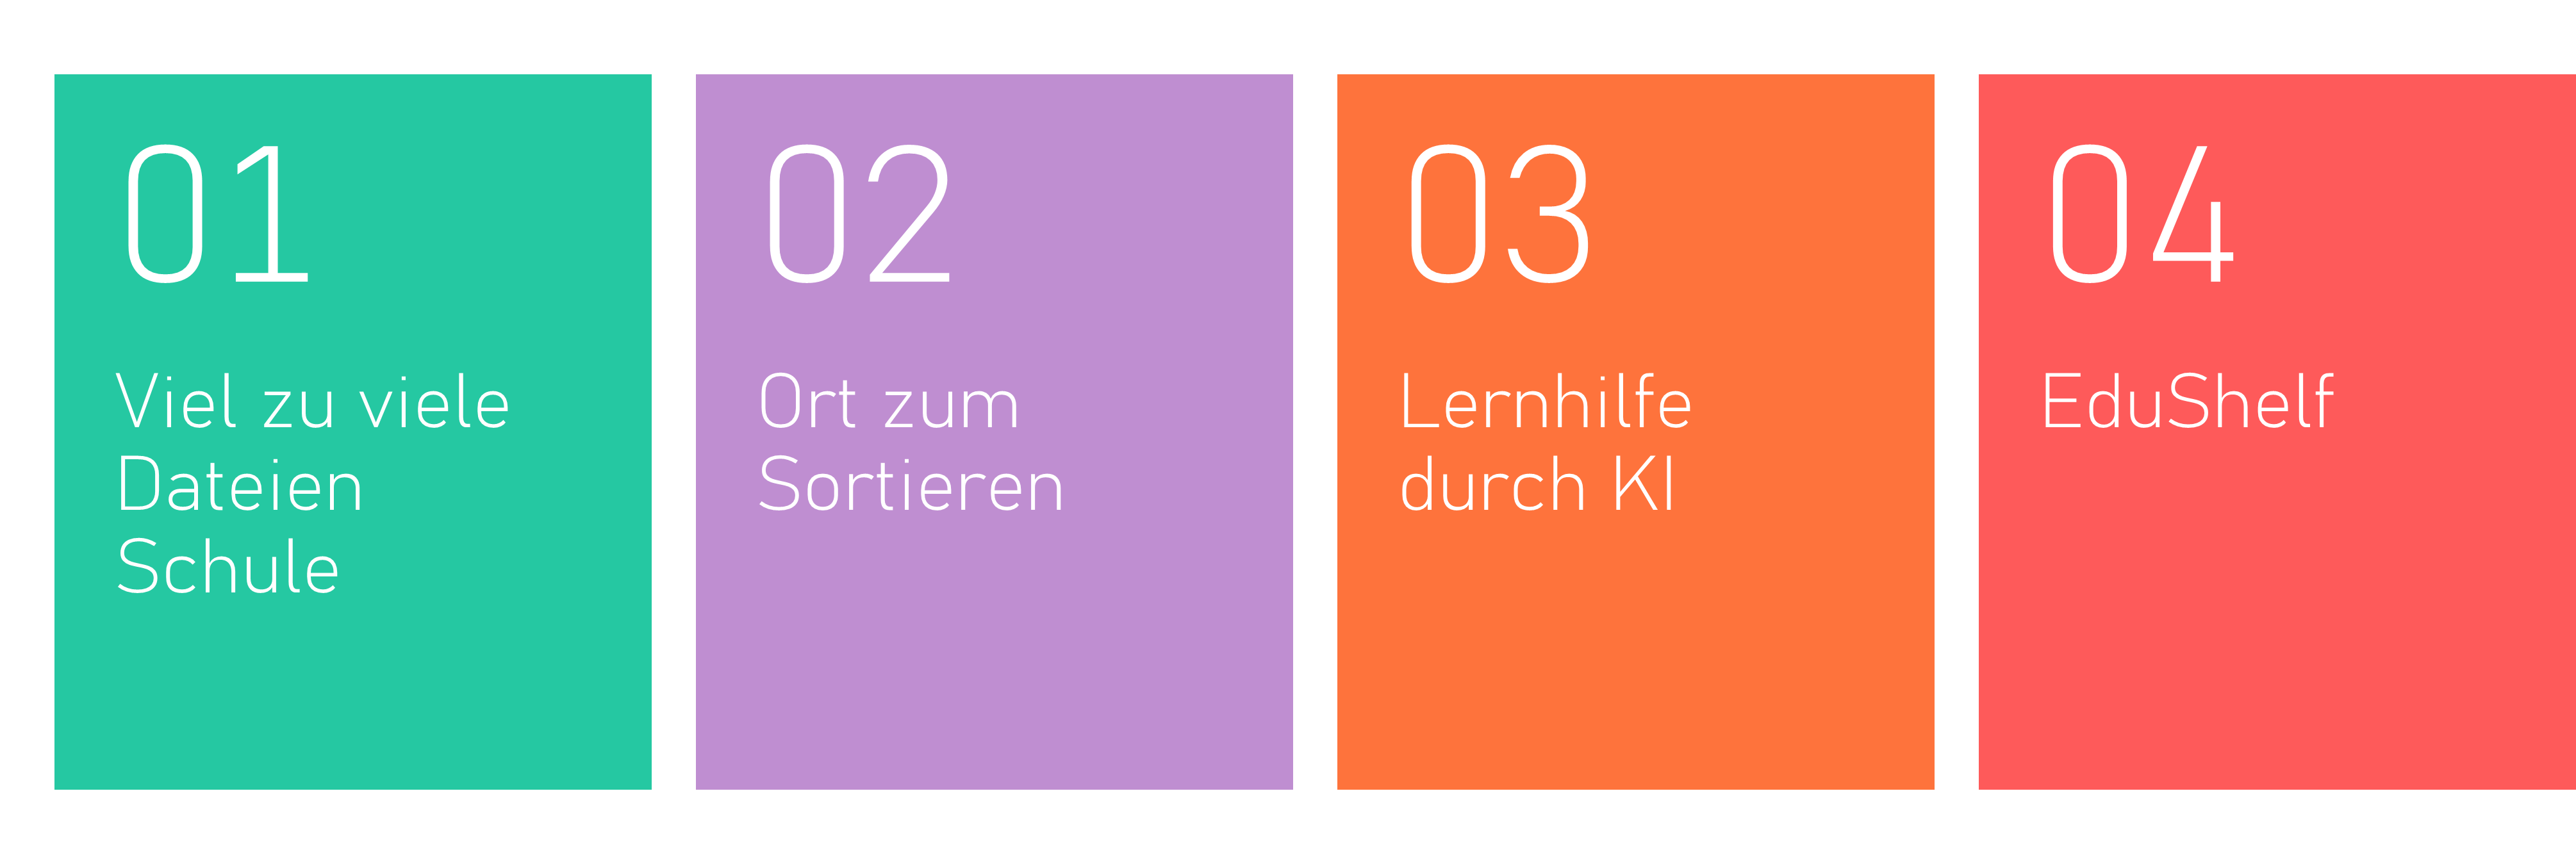
\includegraphics[width=0.85\textwidth]{img/Idee}
    \caption{Konzeptionelle Entwicklung der Idee -- von der Problemerkennung zur Lösung}
    \label{fig:idee}
\end{figure}

\subsection{Stufe 1 -- Problemidentifikation: Unkontrollierter Dateianstieg}

Im schulischen Kontext akkumuliert sich über die Jahre hinweg eine erhebliche Menge an digitalem Lernmaterial. Mitschriften, Übungsblätter, Präsentationen und Abgaben werden typischerweise in heterogenen Strukturen auf verschiedenen Endgeräten oder Cloud-Diensten abgelegt, ohne einer konsistenten Organisationslogik zu folgen. Diese Fragmentierung führt zu einem signifikanten Mehraufwand beim Wiederauffinden relevanter Unterlagen und beeinträchtigt die Effizienz des Lernprozesses nachhaltig. Die erste konzeptionelle Erkenntnis lautet daher: Die schiere Quantität an digitalem Lernmaterial stellt ohne geeignete Verwaltungsstruktur ein wesentliches Produktivitätshemmnis dar.

\subsection{Stufe 2 -- Lösungsansatz: Zentralisierter Speicher- und Sortierort}

Aus der identifizierten Problematik ergibt sich die logische Konsequenz, einen einheitlichen, zentralisierten Ablageort für sämtliche Lernmaterialien zu schaffen. Dieser sollte nicht lediglich als passives Dateisystem fungieren, sondern aktive Mechanismen zur strukturierten Klassifikation und Kategorisierung bereitstellen. Konkret bedeutet dies die Möglichkeit, Dokumente mit beschreibenden Metadaten (Schlagwörter, Fächerzuordnung) zu versehen und gezielt durchsuchbar zu machen. Die Anforderung an einen solchen Speicherort geht folglich über die Funktionalität konventioneller Cloud-Lösungen hinaus, indem eine lernerorientierte Organisationsstruktur in den Mittelpunkt gestellt wird.

\subsection{Stufe 3 -- Erweiterung: KI-gestützte Lernunterstützung}

Die Integration von Methoden der Künstlichen Intelligenz stellt die entscheidende konzeptionelle Erweiterung gegenüber einer reinen Dokumentenverwaltungslösung dar. Die Fähigkeit, auf Basis des individuellen Dokumentenbestands automatisiert Lernhilfen zu generieren -- sei es durch kontextbezogene Fragen und Antworten im Chat-Format, durch das automatische Erstellen von Übungsaufgaben oder durch die Zusammenfassung komplexer Inhalte -- hebt das System auf eine qualitativ höhere Ebene. Dieser Schritt transformiert EduShelf von einem passiven Archiv zu einem aktiven Lernbegleiter, der das gespeicherte Wissen für den Anwender unmittelbar nutzbar macht.

\subsection{Stufe 4 -- Synthese: EduShelf als Gesamtprodukt}

Die vorangehenden drei Erkenntnisstufen münden in der Produktvision von EduShelf. Die Bezeichnung verbindet die Kernfunktionen symbolisch: \textit{Edu} (lat./engl. für Bildung) und \textit{Shelf} (engl. für Regal) verweisen auf einen strukturierten, zugänglichen Wissensraum. EduShelf vereint die zentrale Dateiverwaltung mit intelligenten Lernfunktionen zu einer kohärenten Plattform, die Schülerinnen und Schülern ermöglicht, ihren gesamten Lernprozess -- vom Ablegen der Unterlagen bis zur aktiven Wissensüberprüfung -- in einer einzigen Anwendung zu bündeln. Abbildung \ref{fig:idee} visualisiert diesen Gedankengang als nachvollziehbaren, vierstufigen Prozess von der Problemerkennung bis zur konkreten Produktidee.
